\section{Speed}\label{sectionAcceleration}
The speed is an important parameter in this project. It became important because, in the start of the project, the agent should learn how to accelerate itself. The agent with discrete actions didn't learn the right policy with having the acceleration as a trainable parameter. Acceleration was then changed from a trainable parameter to a constant speed parameter. 

This was done to see if it was possible for the agent to learn how to drive a lap at different speeds. It could be more realistic if it is possible to see the car driving faster than 10 km/h. The tested speed was with an interval of 20 km/h: 
\begin{itemize}
	\item 10 km/h
	\item 30 km/h
	\item 50 km/h
\end{itemize} 

The way the car was driving these average speed, was first the car accelerate to the desired speed – it could be 30 km/h. After this the acceleration is constant, so the speed always stays at 30 km/h. The car will try to stay at the desired speed (30 km/h) the whole lap. For acceleration, the throttle in the environment is the parameter changed. 

To test the speed influence on the trained agent, all other parameters is as described in the introduction to this \Cref{cha:Result}. Thereby it should be possible to only see the influence off the different speeds. 

The most important graph is the graph of the total reward, which looks different from all the speeds, this graph can be seen on \Cref{fig:change_of_acceleration_reward_graph}.

\begin{figure}[H]
	\centering
	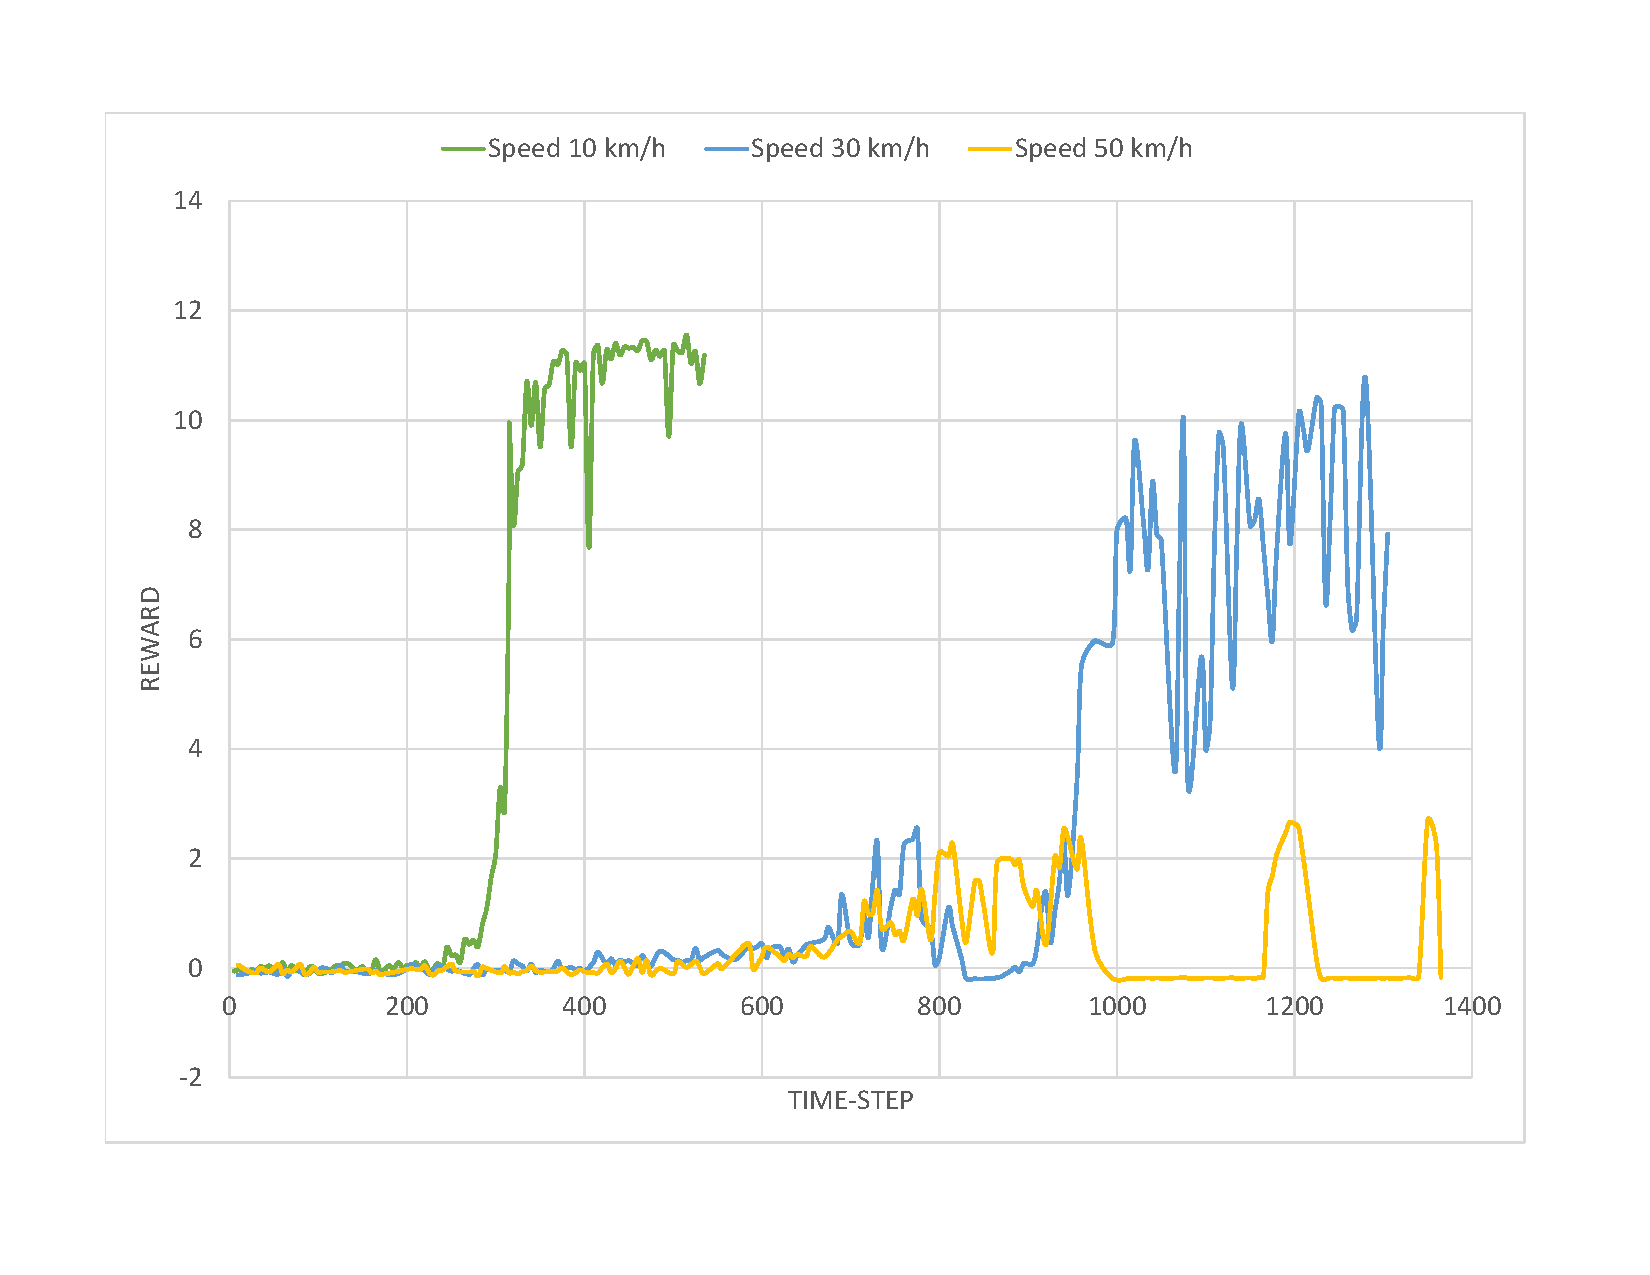
\includegraphics[width=1\textwidth]{Figures/Result/change_of_acceleration_reward_graph.pdf}
	\caption{Comparison of the three different speed with the reward getting from the environment}
	\label{fig:change_of_acceleration_reward_graph}
\end{figure} 

On \Cref{fig:change_of_acceleration_reward_graph}, it is possible to see what happens with the learning on different speeds. By looking at the first speed 10 km/h, it is the speed used in the start of this \Cref{cha:Result}. 

On \Cref{fig:change_of_acceleration_reward_graph}, it is possible to see what happens with the learning on different speeds. By looking at the first speed 10 km/h, it is the speed used in the start of this \Cref{cha:Result}. 

To compare a speed of 10 km/h with a speed of 30 km/h the agent seems to learn how to drive at booth speeds, seen by both speeds conjugate at some reward. A speed of 10 km/h conjugates around a reward of 11, and a speed of 30 km/h around a reward of 8. The different reward value is because of the different speeds, due to the speed is taken into account when calculation the reward - in the reward function seen in \Cref{sectionReward}. 

The speeds of 10 km/h and 30 km/h have different stabilities, as a speed of 10 km/h looks to be more stable around a reward of 11. With the speed of 30 km/h, the reward seems to be unstable because it is not as constant around a reward of 8 as a speed of 10 km/h is a reward of 11.

By looking at the training time of the two speeds 10 km/h and 30 km/h, it looks like a speed of 10 km/h is learning faster. It is learning faster in time-steps because it doesn't need as many time-steps as a speed of 30 km/h to learn. But every time-step is ended faster with a speed of 30 km/h, then with a speed of 10 km/h, this is due to the time of the time-steps. As mentioned earlier a time-step ends, when the car drives out of the track, the car drives backward or the car finishes a lap. With having a speed of 30 km/h the car will drive faster, and thereby will the time-steps be shorter. To compare the training time the graph on \Cref{fig:change_of_acceleration_reward_graph} isn't sufficient, so another graph with hours instead of time-steps is created and can be seen on \Cref{fig:change_of_acceleration_reward_hours_graph}.

\begin{figure}[H]
	\centering
	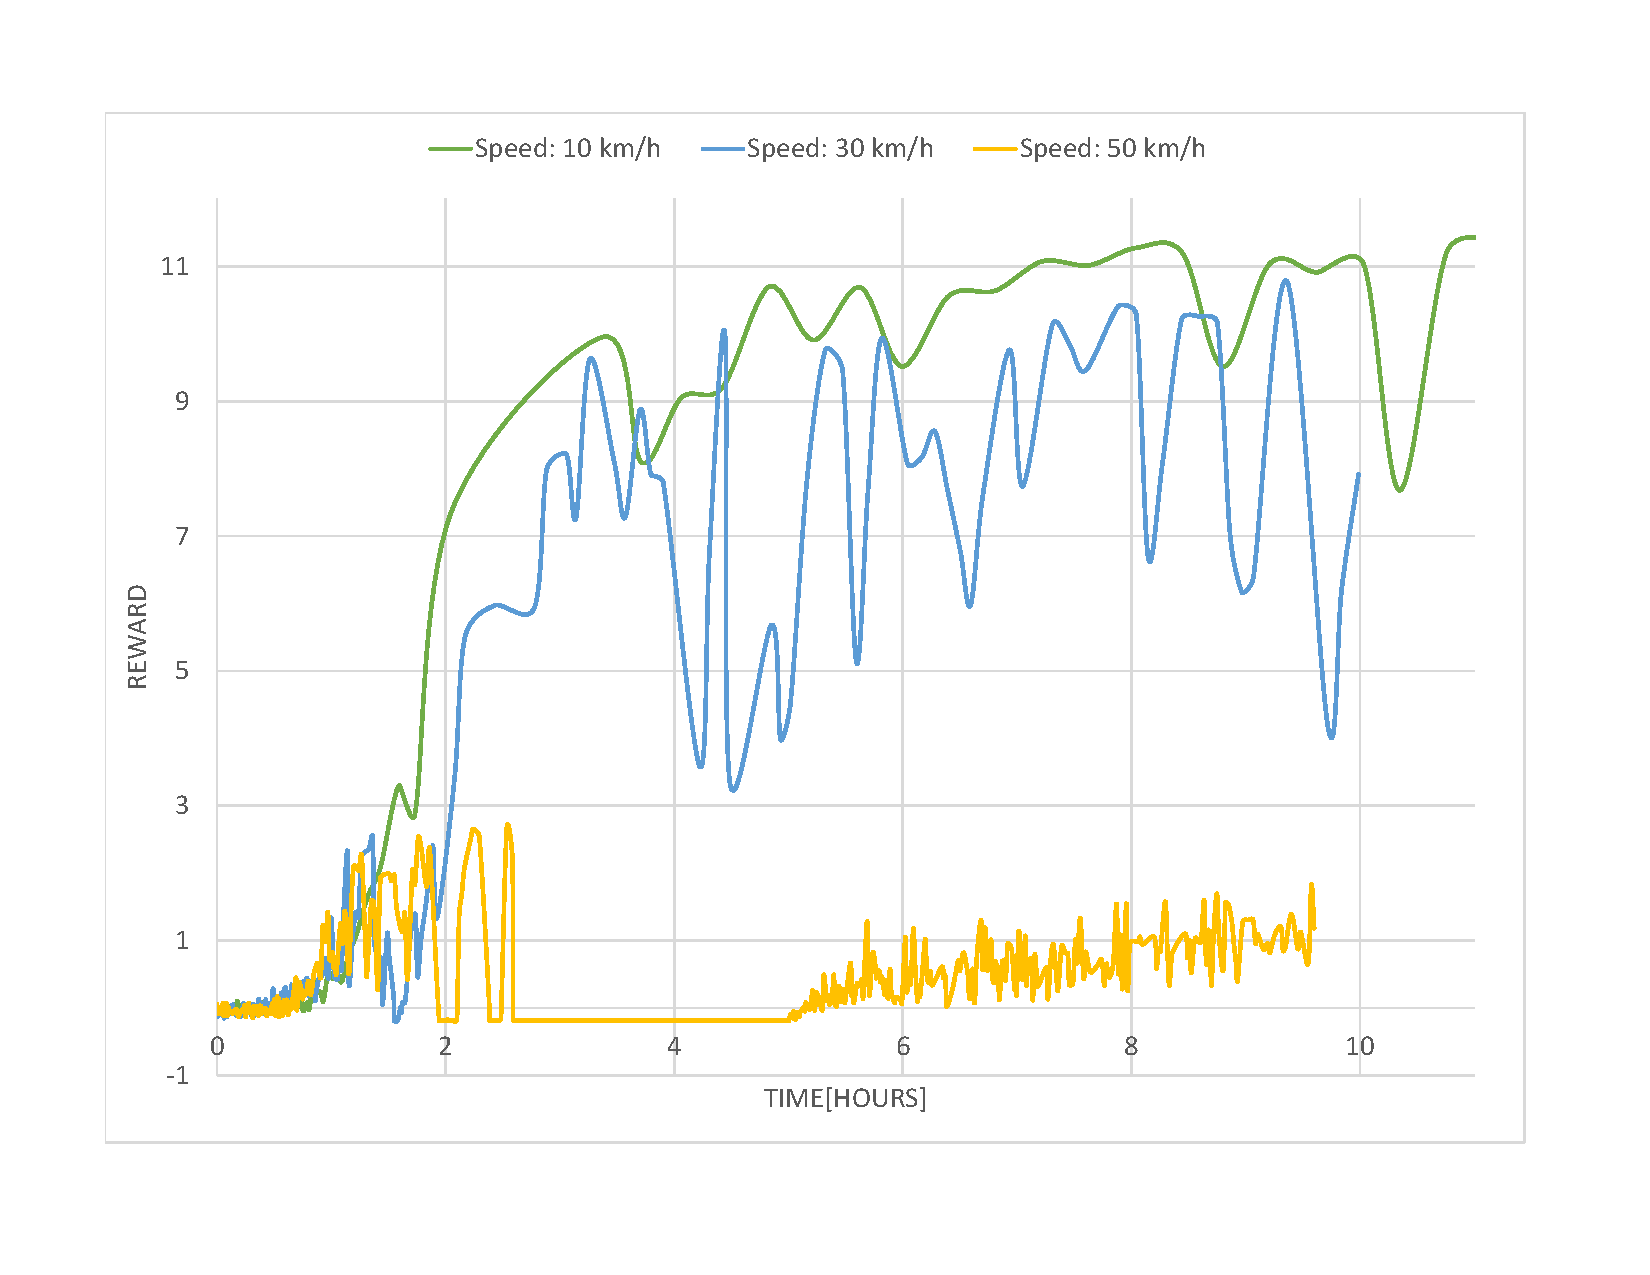
\includegraphics[width=1\textwidth]{Figures/Result/change_of_acceleration_reward_hours_graph.pdf}
	\caption{Comparison of the three different speed with the reward getting from the environment. Here it is the time in hours, instead of time-steps on the x-axis}
	\label{fig:change_of_acceleration_reward_hours_graph}
\end{figure}

\Cref{fig:change_of_acceleration_reward_hours_graph} shows that the learning time in hours is close to being the same, for both a speed of 10 km/h and 30 km/h. Both speeds conjugate after 3 hours of training, thereby there no difference in the learning time for 10 km/h and 30 km/h.

By looking at the learned agent driving in the TORCS environment, it is seen that at 10 km/h and 30 km/h has learned how to drive a lap. It is easy to see that the stability at a speed of 30 km/h is not as good as the stability with a speed of 10 km/h. The car on 30 km/h makes bigger turns, which means it gets closer to the edge. The 10 km/h drives more smoothly in the center of the road.

As seen on both \Cref{fig:change_of_acceleration_reward_graph} and \Cref{fig:change_of_acceleration_reward_hours_graph} the agent doesn't learn how to drive with a speed of 50 km/h. It never conjugates to the best reward, it seems that it is learning something but never continues learning. After looking at the agent in the TORCS environment it is also seen that the agent doesn’t learn how to drive a lap.

The problem with not learning at a speed of 50 km/h, could be due to the discrete values for steering send as a discrete action. This discrete action could be adjusted to the different speed because with the higher speed the steering has more influence on the car than on lower speeds. This could maybe also solve the problem of the stability with a speed of 30 km/h. 

The conclusion by looking at the results from the different speeds is that the agent performs better at a speed of 10 km/h and thereby is the used speed for another testing.

    